\section{Tricks}

In this section are described random tricks used to speed up rendition. They range from simple cos/sin offset to what I consider one of the most beautiful hack in the engine: Linear Feedback Shit Register.




\subsection{Cos/Sin table}
\cw{cos} and \cw{sin} are expensive methods but they are heavily used at runtime. So speed things up the engine generates and precache them at startup and store them in a lookup array (one value per angle). But it does so in a smart way: It exploit a math property ($cos(X) = sin(X + 90)$) to avoid 360 \cw{sin} method calls and 240 bytes of RAM by reusing the cos table as follow:\\
\par

\begin{minipage}{\textwidth}
\lstinputlisting[language=C]{code/sin_cos_table.c}
\end{minipage}


\begin{figure}[H]
 \centering
  \includegraphics[width=\textwidth]{imgs/drawings/cos_sin_table.pdf}
 \caption{Finalez frame} 
\end{figure}








\subsection{FizzleFade}
While most screen transition are done with a black fade effect (by shifting the palette), there are two instances
when the screen transition via fizzling:
\begin{itemize}
	\item When dying
	\item When killing a boss
\end{itemize}




\begin{minipage}{\textwidth}
\centering
  \scaledimage{.9}{fizzlefade/dying/screenshot_16.png}\\
  \vspace*{0.5cm}
  \scaledimage{.9}{fizzlefade/dying/screenshot_19.png}\\
\end{minipage}

\begin{minipage}{\textwidth}
\centering
  \scaledimage{.9}{fizzlefade/dying/screenshot_52.png} \\
  \vspace*{0.5cm}
  \scaledimage{.9}{fizzlefade/dying/screenshot_86.png} \\
\end{minipage}


\begin{minipage}{\textwidth}
\centering
  \scaledimage{.9}{fizzlefade/boss/screenshot_60.png} \\
  \vspace*{0.5cm}
  \scaledimage{.9}{fizzlefade/boss/screenshot_66.png}  \\
\end{minipage}

\begin{minipage}{\textwidth}
\centering
  \scaledimage{.9}{fizzlefade/boss/screenshot_102.png}\\
\vspace*{0.5cm}
  \scaledimage{.9}{fizzlefade/boss/screenshot_130.png}\\
\end{minipage}

A naive approach would have been to reuse the pseudo random generator \cw{US\_RndT} and keep track of which pixels had been fizzled. But that would make the fade non-deterministic with regard to duration and that would also be a waste of CPU cycles since a same pixel coordinate (X,Y) could come up several times.\\
\par
It turns out there is a much faster and elegant way to do it. The code responsible for this effect can be found in id\_vh.cpp, function FizzleFade. It is in my humble opinion one of the most beautiful hack in Wolfenstein 3D. At first it is not obvious to understand how it works:\\
\par
\begin{minipage}{\textwidth}
\lstinputlisting[language=C]{code/fizzlefade.c}
\end{minipage}
\par
Which can be read as:\\
\begin{itemize}
\item Initialize \cw{rndval} to 1.
\item Break it down in 8 + 7 bits: Use 8 bits generate an X coordinate and 7 bits for a Y coordinate.
\item Subject \cw{rndval} to a soup of XORing.
\item When \cw{rndval} value is somehow back to 1: Stop.
\end{itemize}        
It looks like magic at first. How is \cw{rndval} supposed to be back to 1?! This technique is called Linear Feedback Shit Register. To make it work, one needs a register which will be right shifted each iteration. Since it is right shited, the right bit dissapear and a new one to the left is needed.\\
TODO:DRAWING\\
\par
To generate this new bit we introduce "taps" which are bit offset used to XOR together values and generate the new bit value\\
TODO:DRAWING\\
\par
A Fibonnaci representation shows a simple LFSR with one tap:\\
TODO:DRAWING\\
\par
TODO:VALUES\\
\par
A slightly more complex one with two registers:\\
TODO:DRAWING\\
\par
TODO:VALUES\\

\par

\begin{figure}[H]
 \centering
  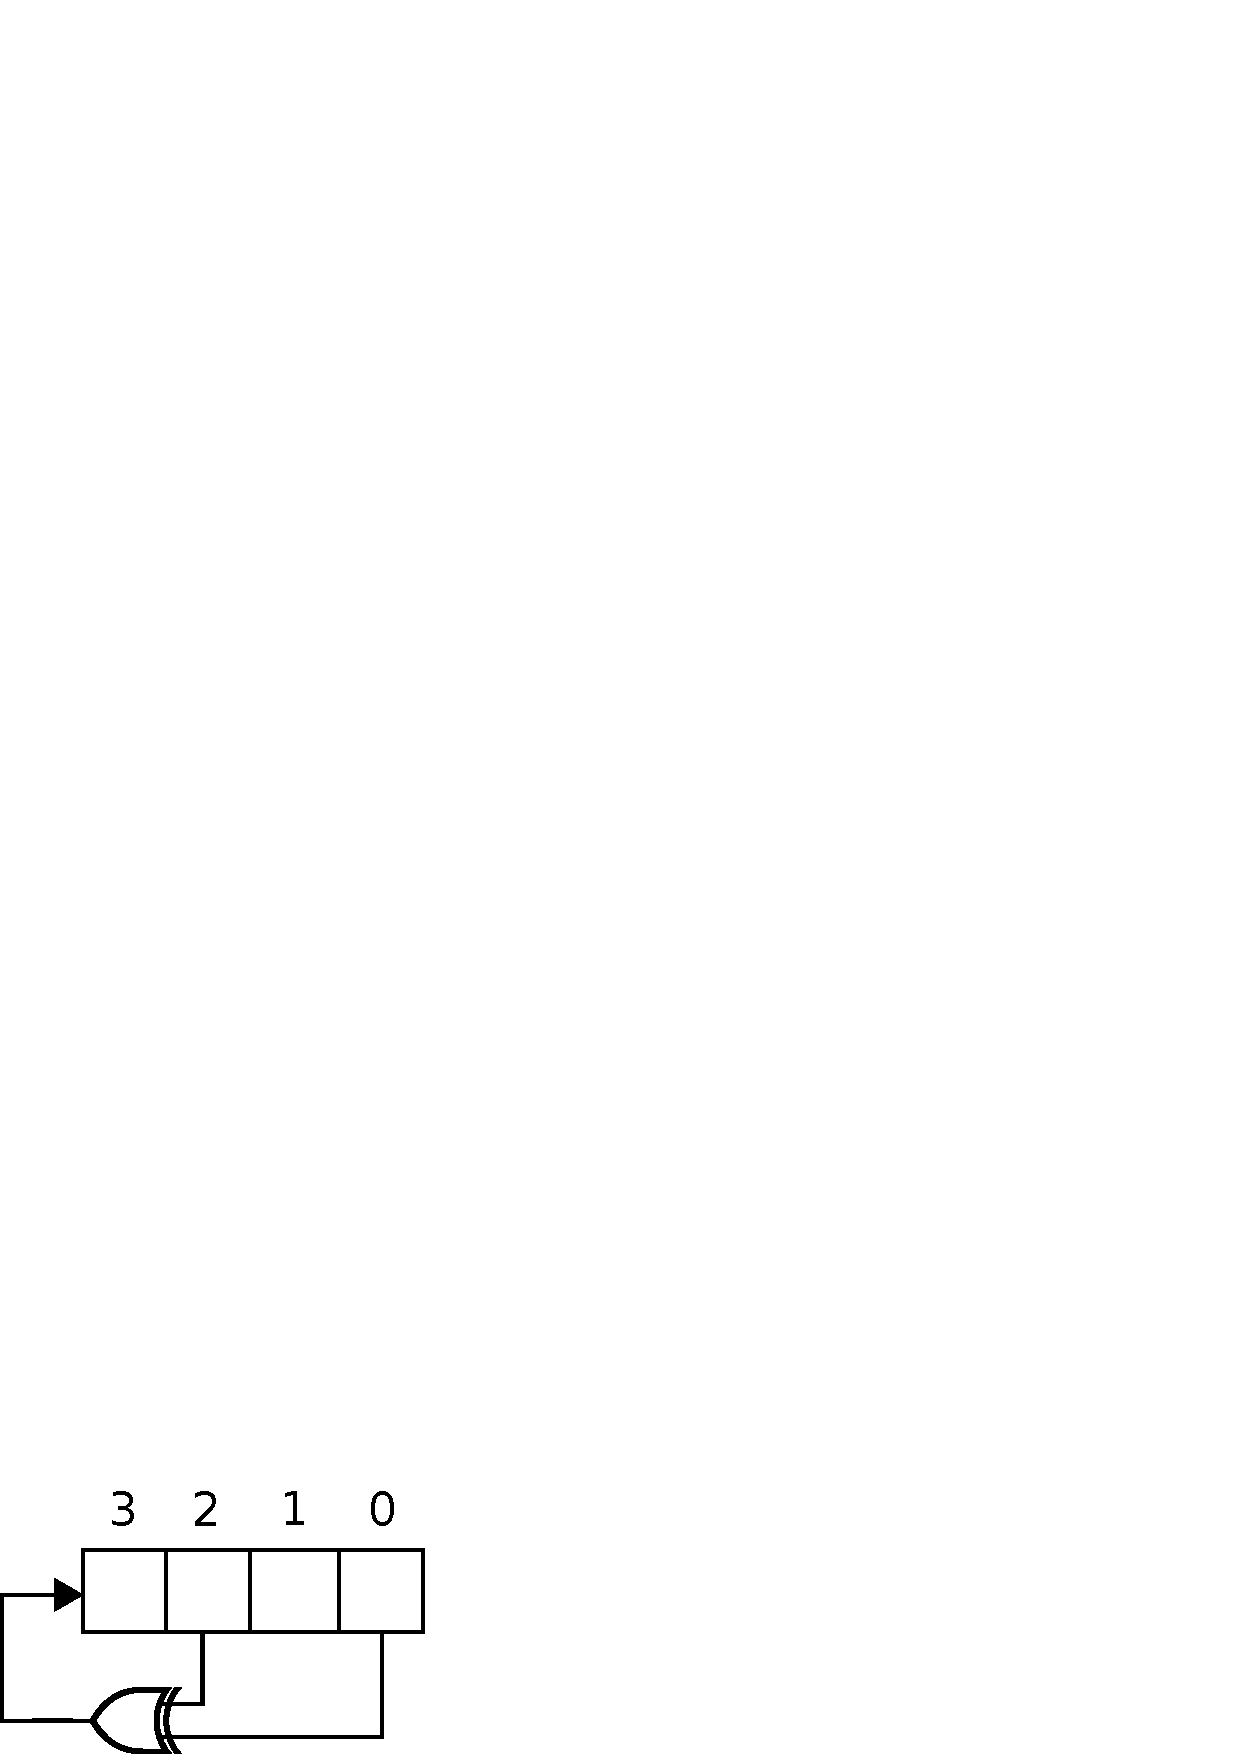
\includegraphics[width=.4\textwidth]{imgs/drawings/4bits_lfsr.pdf}
 \caption{Finalez frame} 
\end{figure}

\par
\begin{minipage}{\textwidth}
\lstinputlisting[language=C]{code/lfsr.txt}
\end{minipage}
\par

\begin{figure}[H] \centering \includegraphics[width=\textwidth]{imgs/drawings/fizzlefade/fibonacci.pdf} \end{figure}
\begin{figure}[H] \centering 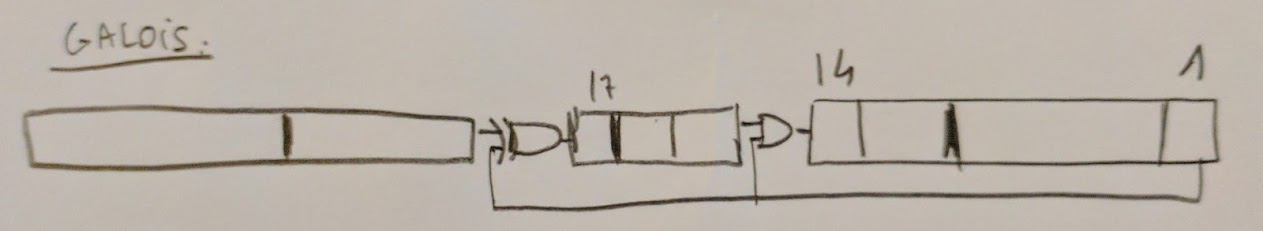
\includegraphics[width=\textwidth]{imgs/drawings/fizzlefade/galois.pdf} \end{figure}
      
Note: Because the effect works by plotting pixels individually, this effect was very hard to replicate when developers tried to port the game to hardware accelerated GPU. As far as I know none of the port managed to replicate the fizzlefade.

Note: If you are curious about maximum-length taps, xilinx provides them from 3 to 168\footnote{Xilinx table can be found \href{http://www.xilinx.com/support/documentation/application\_notes/xapp052.pdf}{here}.}.










\subsection{Palette}
Even though it limit the graphic capabilities, the palette system can be turned into a strength: It is easy to fade the screen to white (when picking up an item) or red (when taking damages).\\
It only takes 256*3 = 768 bytes and 768 out instructions to modify the full screen:
\begin{figure}[H]
  \centering
 \fullimage{palette_damage.png}
 \caption{The palette RGB colors altered when taking damage.} \label{fig:palette_damage}
\end{figure}
A fast path is provided (which ironically only works if the CPU is as slow at the VGA) to update the palette via one \cw{lobsb} instruction. Otherwise if not supported a loop of 768 \cw{outsb} is used.\\
\par
\begin{minipage}{\linewidth}
\lstinputlisting[language=C,morekeywords={asm,byte,far}]{code/vl_setpalette.c}
\end{minipage}








\section{Pseudo random generator}

\begin{minipage}{\textwidth}
\lstinputlisting[language={[x86masm]Assembler}, style=mystyle,basicstyle=\small]{code/rndtable.asm}
\end{minipage}

\begin{minipage}{\textwidth}
\lstinputlisting[language={[x86masm]Assembler}]{code/US_InitRndT.asm}
\end{minipage}


\begin{minipage}{\textwidth}
\lstinputlisting[ language={[x86masm]Assembler}]{code/US_RndT.asm}
\end{minipage}








